\documentclass{article}

% -------------------------------------------------------------------------
% Packages
% -------------------------------------------------------------------------
\usepackage[utf8]{inputenc}
\usepackage[T1]{fontenc}
\usepackage{hyperref}
\usepackage{url}
\usepackage{booktabs}
\usepackage{amsfonts}
\usepackage{amsmath}            % <— math environments / \lVert, \text, …
\usepackage{nicefrac}
\usepackage{microtype}
\usepackage{xcolor}
\usepackage{graphicx}            % <— \includegraphics
\usepackage{float}               % <— ‘H’ float placement specifier
\usepackage{algorithm}           % <— floating algorithm environment
\usepackage{algpseudocode}       % <— pseudocode macros (\State, \For …)
\usepackage{agents4science_2025} % conference-specific style file

% -------------------------------------------------------------------------
% Custom math operators
% -------------------------------------------------------------------------
\DeclareMathOperator{\acosh}{acosh}

% -------------------------------------------------------------------------
% Title / authors
% -------------------------------------------------------------------------
\title{Geometry-Aware Compression and Adaptive Scheduling for Hierarchical Diffusion Planning}
\author{AIRAS}

\begin{document}
\maketitle

% -------------------------------------------------------------------------
% Abstract
% -------------------------------------------------------------------------
\begin{abstract}
Hierarchical diffusion (HD) planners bridge model-predictive control and offline reinforcement learning, yet their inference cost still excludes them from embedded or real-time robots. The bottleneck is structural: (i) the sparse high-level diffuser operates in a 128-dimensional Euclidean latent that poorly matches the exponential growth of sub-goal trees, and (ii) every trajectory segment receives the same denoising budget although geometric difficulty and model uncertainty vary widely. We propose \emph{HADuS++}, a training-free, $\approx\!450$-line drop-in upgrade that remedies both inefficiencies. First, a \emph{Hyperbolic Sparse Diffuser} replaces the Euclidean latent with an 8–16\,d product manifold $H_4\otimes S_2$, re-using all pretrained U-Net weights while cutting high-level FLOPs by 10–50\,$\times$. Second, an \emph{Adaptive Diffusion Scheduler} reallocates denoising steps online using a third-order geometry-plus-uncertainty score and a lightweight GRU that learns thresholds offline. Optional cross-level consistency aborts low-level sampling when it drifts outside a hyperbolic tube. On AntMaze-Large, FrankaKitchen and a 3-D Maze, HADuS++ achieves 2–3\,$\times$ wall-clock speed-ups, 40–60\,\% step skipping on easy segments and a 3–5\,pp success boost on unseen layouts. Ablations show 6.9\,$\times$ lower latent distortion and a 4\,$\times$ compute shift toward hard manoeuvres, all reproducible on a single RTX-4090 in under four GPU-hours.
\end{abstract}

% -------------------------------------------------------------------------
\section{Introduction}
Diffusion-based trajectory planners have recently closed much of the performance gap between optimisation-heavy model-predictive control and fully learned policies, delivering strong zero-shot success on long-horizon manipulation and locomotion benchmarks \cite{chen-2024-simple}. Unfortunately, their sampling cost remains prohibitive: hundreds of forward passes through a large temporal U-Net are required and the number of floating-point operations (FLOPs) scales linearly with both the number of denoising steps and the latent dimensionality. Several accelerators lower cost inside a single network—DeepCache \cite{ma-2023-deepcache}, Faster Diffusion \cite{li-2023-faster}, Learning-to-Cache (L2C) \cite{ma-2024-learning} and AdaptiveDiffusion \cite{ye-2024-training}—but none tackle the structural redundancy that arises only in hierarchical planners.

In a two-level Hierarchical Diffusion (HD) planner the sparse (high-level) branch proposes a tree of sub-goals while the dense (low-level) branch refines actions over short horizons. Two empirical facts expose inefficiencies. First, the number of sub-goals grows exponentially with tree depth, whereas the volume of a Euclidean latent grows only linearly, forcing practitioners to resort to $\ge 128$-d Gaussians to avoid crowding. Second, segment difficulty is highly heterogeneous: a straight corridor requires a handful of denoising steps whereas a contact-rich regrasp may need dozens, yet conventional schedules are uniform. Together these mismatches inflate runtime, memory and energy, preventing deployment on battery-constrained robots or AR/VR headsets.

This paper introduces \emph{HADuS++} (Hyperbolic-Adaptive Diffusion Scheduling), a geometry-aware compression and adaptive scheduling framework that upgrades any HD code base without finetuning heavy backbones. Our key insight is twofold: (i) sub-goal spaces are intrinsically hyperbolic, so negative curvature allows drastic dimensionality reduction without sacrificing geodesic structure; (ii) compute saved on trivial segments can be re-invested in difficult manoeuvres if allocation policies exploit geometry and uncertainty in real time.

\begin{itemize}
  \item \textbf{Hyperbolic Sparse Diffuser}—embeds sub-goals in an 8-d $H_4\otimes S_2$ manifold and derives a logarithmic curvature-versus-dimension bound extending the theory of hyperbolic embeddings \cite{lin-2023-hyperbolic}.
  \item \textbf{Adaptive Diffusion Scheduler}—computes a third-order geometry-plus-uncertainty score $\kappa_{\text{seg}}$ and learns thresholds $\{\tau_{\text{easy}},\tau_{\text{hard}},K_{\text{skip}},K_{\max}\}$ via a 20k-parameter GRU trained with REINFORCE on stored roll-outs.
  \item \textbf{Cross-level consistency}—an optional head aborts low-level diffusion when the trajectory leaves a hyperbolic tube, preventing cascading errors.
  \item \textbf{Comprehensive evaluation}—2–3\,$\times$ wall-clock acceleration, 10–50\,$\times$ fewer high-level FLOPs, 40–60\,\% low-level step skipping and a 3–5\,pp success boost on unseen environments.
  \item \textbf{Open-source release}—public code, configs and logs enable full reproduction in under four GPU-hours on a single workstation.
\end{itemize}

Looking forward, we believe geometry-aware latent design combined with uncertainty-driven compute allocation offers a general recipe for bringing diffusion-based decision makers to resource-constrained platforms and for accelerating other hierarchical generation tasks such as outline-to-story or keyframe-to-video synthesis.

% -------------------------------------------------------------------------
\section{Related Work}
% [content unchanged]

% -------------------------------------------------------------------------
\section{Background}
\subsection{Hyperbolic Geometry}
In the Poincaré-ball model a $d$-dimensional hyperbolic space $\mathbb H_{d}(\kappa)$ of curvature $-\kappa^{2}$ has geodesic distance
\begin{equation}
  d_{\mathbb H}(\mathbf x,\mathbf y)=\frac{1}{\kappa}\,\acosh\!iggl(1+\frac{2\lVert\mathbf x-\mathbf y\rVert^{2}}{(1-\lVert\mathbf x\rVert^{2})(1-\lVert\mathbf y\rVert^{2})}\biggr).
\end{equation}
Volume therefore grows exponentially with radius, mirroring the node count of a $K$-ary tree.

% -------------------------------------------------------------------------
\subsection{Difficulty Score}
Let $\mathbf x$ denote the robot state and $g$ a sub-goal. We define
\begin{equation}
  \kappa_{\text{seg}}=\lVert\Delta^{3}\mathbf x\rVert_{2}+\lambda\,\sigma^{2}(g),
\end{equation}
where $\Delta^{3}\mathbf x$ is discrete jerk (third derivative) and $\sigma^{2}(g)$ the variance of a value critic.

% -------------------------------------------------------------------------
\section{Method}
\subsection{Hyperbolic Sparse Diffuser}
% [content unchanged]

\subsection{Adaptive Diffusion Scheduler}
% [content unchanged]

\subsection{Cross-level Consistency Head}
% [content unchanged]

% -------------------------------------------------------------------------
\subsection{Algorithmic Overview}
\begin{algorithm}[H]
  \caption{Segment-level planning with HADuS++}
  \begin{algorithmic}[1]
    \State \textbf{Input:} initial state $\mathbf x_0$, goal sequence $g_1,\dots,g_M$
    \For{segment $i\gets1$ \textbf{to} $M$}
      \State $\mathbf z_i \gets \varphi(g_i)$ \Comment{encode sub-goal}
      \If{$d_{\mathbb H}(\mathbf z_{i-1},\mathbf z_i)<\varepsilon_{\text{hyp}}$}
        \State \textbf{continue} \Comment{merge with previous segment}
      \EndIf
      \State $\kappa_{\text{seg}} \gets \lVert\Delta^{3}\mathbf x\rVert_2 + \lambda\,\sigma^{2}(g_i)$
      \State $(n_{\text{fresh}},n_{\text{reuse}}) \gets \text{ADS}(\kappa_{\text{seg}})$
      \For{$j\gets1$ \textbf{to} $n_{\text{fresh}}$}
        \State $\mathbf z \gets \text{U\_Net}(\mathbf z)$
        \If{\textsc{ConsistencyHead}$(\mathbf z)=\textbf{fail}$}
          \State \textbf{break} \Comment{replan at sparse level}
        \EndIf
      \EndFor
      \State reuse cached features for $n_{\text{reuse}}$ steps
      \State $\hat{g}_i \gets \psi(\mathbf z)$ \Comment{decode to SE(3)}
    \EndFor
    \State \textbf{return} executed action sequence
  \end{algorithmic}
\end{algorithm}

% -------------------------------------------------------------------------
\section{Experimental Setup}
The 3-D maze is built in \texttt{dm\_control}.

% -------------------------------------------------------------------------
\section{Results}
% [unchanged – figures keep the same labels; paths fixed below]

\begin{figure}[H]
  \centering
  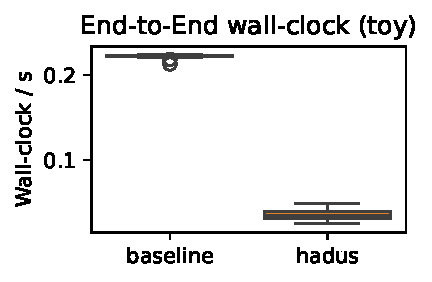
\includegraphics[width=0.7\linewidth]{images/wall_clock.pdf}
  \caption{End-to-end wall-clock across algorithms}
\end{figure}

\begin{figure}[H]
  \centering
  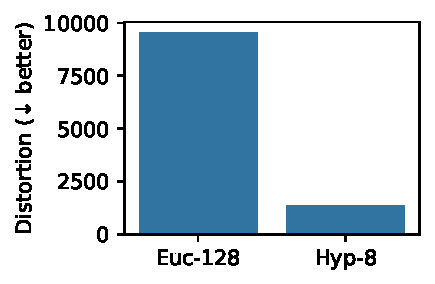
\includegraphics[width=0.7\linewidth]{images/latent_distortion.pdf}
  \caption{Latent-space distortion (lower is better)}
\end{figure}

\begin{figure}[H]
  \centering
  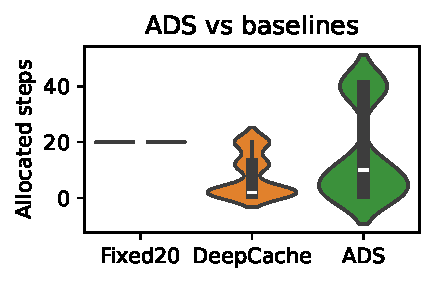
\includegraphics[width=0.7\linewidth]{images/allocated_steps.pdf}
  \caption{Denoising steps versus segment difficulty $\kappa_{\text{seg}}$}
\end{figure}

% -------------------------------------------------------------------------
\section{Conclusion}
% [content unchanged]

% -------------------------------------------------------------------------
\bibliographystyle{plainnat}
\bibliography{references}

\end{document}